\documentclass{book}

\usepackage[ISSUE]{liltcsli}
\usepackage{longtable}

%\raggedbottom   % Uncomment this line if large diagrams cause vertical gaps.

\hfuzz = 2pt     % No warnings about margin overhangs less than this amount.

%\crop[]         % Uncomment for centered pages.
%\crop[cam]      % Uncomment for crosshairs that show corners of each page.
%\crop[frame]    % Uncomment for rectangle that shows edges of each page.


\usepackage[comma]{natbib}  % CSLI Pubs favored bibliography package.
\usepackage{chapterbib}     % Makes a section out of References

\usepackage{booktabs}

% Create your own separate style file and load here to avoid cluttering
% up the preamble more than necessary.  There should be no definitions,
% etc. after the \begin{document} command.
%\usepackage{mymacros}
%\usepackage{times}
\usepackage{latexsym}
\usepackage{epsfig}
\usepackage[latin1]{inputenc}
\usepackage[T1]{fontenc}
%usepackage{pslatex}
%\usepackage{rotating}
\usepackage[english]{babel}
\selectlanguage{english}
%%\usepackage{makeidx,color}
\usepackage{gb4e}
\usepackage{amsfonts}


\volumeissue {1}{to be filled in}
\monthyear   {to be filled in}{2014}
%each issue is one article
\title       {A computational analysis of poetic style}
\subtitle{Imagism and its influence on modern professional and amateur poetry}
\author      {Justine T. Kao\affiliation{Department of Psychology, Stanford University} {Dan Jurafsky\affiliation{Department of Linguistics, Stanford University}}}

\begin{document}

\section*{Abstract}
How do standards of poetic beauty change as a function of time and expertise? Here we use computational methods to compare the stylistic features of poems written by 19th century professional poets, contemporary professional poets, and contemporary amateur poets. Building upon techniques designed to analyze style and sentiment in texts, we examined elements of poetic craft such as imagery, sound devices, emotive language, and diction. We found that contemporary professional poets used significantly more concrete words than 19th century poets, fewer emotional words, and more complex sound devices. These changes are consistent with the tenets of Imagism, an early 20th-century literary movement. Further analyses showed that contemporary amateur poets resembled 19th century professional poets more than contemporary professional poets on these dimensions, suggesting that elite standards of poetic beauty in the past ``trickled down'' to influence amateur works in the present. Our results highlight the influence of Imagism on the modern aesthetic and reveal the dynamics between ``high'' and ``low'' art. We suggest that computational linguistics may shed important light on the forces and trends that shape poetic style.

\clearpage

\section{Introduction} 
From Homer's epics, to Li Po's elegant verses, to Billy Collins' charming and often startling portraits of everyday life, poetry has been widely celebrated across languages, cultures, and time. Countless readers have experienced the power of a beautiful poem; however, an astute reader will notice that this power takes a different form in Shakespeare's measured sonnets than it does in Pablo Neruda's lush poetry. In this paper, we are interested in the forces and elements that shape the aesthetic standards of poetry. In particular, how do literary movements transform ideals of poetic beauty? How do changes in aesthetic standards impact poets with high versus low levels of expertise? Can we characterize this transformation using precise quantitative methods and analyze its influence on a large scale? 

%\subsection{Artistic change}
Many literary critics, historians, and social scientists have studied artistic change and proposed theories about its inception and development. These scholars have approached artistic change from the perspective of direct influence among artists \citep{clayton1991influence},  legitimation of new or previously ignored art forms due to social change \citep{baumann2007general}, and the dynamics between high and low social classes \citep{simmel1957fashion}. This diversity of approaches suggests that a holistic view of artistic change should incorporate the influence of individual artists as well as more general forces such as class dynamics or the nature of artistic appreciation itself. While the ideas proposed in these works are enlightening and influential, their methods have been mostly qualitative, making it difficult to draw objective and data-driven conclusions about large bodies of texts.

 \cite{martindale1990clockwork} was one of the first to use quantitative methods to comprehensively analyze a sizable collection of artwork across several time periods. His analysis showed that visual, verbal, and musical art all tend to exhibit higher complexity over time, suggesting that a major force for artistic change may be the pressure to be less predictable and thus more complex. While this research presents compelling quantitative evidence to support a theory of artistic change, it (largely intentionally) ignores the  historical context in which change takes place. Furthermore, Martindale regards certain types of art such as poetry as a product of the elite and overlooks poetry generated and consumed by the masses. While this approach sheds light on broad patterns of artistic change, it fails to consider the different ways in which the force of change acts upon artists in different historical and social contexts.

In this paper, we apply the same degree of quantitative rigor to examine changes surrounding a specific literary movement: Imagism. By focusing on a particular movement, we are able to examine whether and how powerful literary leaders can dramatically shift the standards of poetic beauty within a short amount of time. Furthermore, by comparing the movement's effect on elite poets and amateur poets, we aim to explore the differences between high and low art and their responsiveness to change. 

We chose to focus on the Imagist movement for two reasons. First, Imagism is regarded by many literary critics as ``the beginning of modern literature in English'' \citep{pratt1992imagism}. Leaders of the Imagism movement articulated and championed some of the principles of craft still taught in creative writing workshops today, such as the advice to show and not tell \citep{PoetsCompanion, Burroway}. If the Imagism movement has such a strong influence on modern aesthetic standards, then we should find significant differences between the styles of poems written prior to and following the movement. Second, while the work of amateur poets before the 21st century is mostly undocumented, the Internet now enables easy dissemination and documentation of poems produced by the masses. It is now possible to collect poems not only from modern anthologized poets, but also from modern amateur poets who published their work on the Internet. By choosing a movement closer to our times, we are able to compare the influence of Imagism on poems written by poets with vastly different levels of skills and formal training. 

\subsection*{The Imagist movement}

Given its significance, the Imagism movement was surprisingly small and short-lived. The movement officially launched in 1912 and ended in 1917, involving only a handful of English and American poets, including Ezra Pound, Amy Lowell, William Carlos Williams, and James Joyce. Ezra Pound is regarded as the intellectual leader of the movement (although Amy Lowell took over soon afterwards, not without some drama). Although there are speculations about Pound's personal motives for launching the movement \citep{thacker2011imagist}, Imagism is often construed as a reaction against Georgian and Victorian styles, which are characterized by abstract and sentimental language \citep{frank1991idea}. The Imagists articulated their aesthetic ideals in an anthology published in 1916, titled ``Some Imagist Poets.'' Here we list the six tenets they proposed, modified for brevity:
\begin{itemize}
\item[1.] To use the language of common speech, but to employ always the exact word, not the nearly-exact, nor the merely decorative word.
\item[2.] To create new rhythms---as the expression of new moods---and not to copy old rhythms, which merely echo old moods. 
\item[3.] To allow absolute freedom in the choice of subject.
\item[4.] To present an image. We believe that poetry should render particulars exactly and not deal in vague generalities.
\item[5.] To produce poetry that is hard and clear, never blurred nor indefinite.
\item[6.] Finally, concentration is of the very essence of poetry.
\end{itemize}

Pound's poem titled \emph{In a Station of the Metro}, published in \emph{Poetry} magazine in 1913, embodies the central tenets of the Imagism movement:

\begin{verse}
\emph{The apparition of these faces in the crowd;\\
Petals on a wet, black bough.}
\end{verse}

In fourteen words, the poem constructs a clear and compelling image that conveys an abstract emotional experience without explicitly describing it. The poem does not follow a strict meter or rhyme scheme; instead, the relationship between the two lines is one of imagery rather than one of sound. The image of faces in the crowd is equated with an image of petals on a bough, remnants of flowers that had just been separated from the tree after rain. A sense of ephemerality is evoked by the precise and concrete image of these delicate petals, which lingers in the reader's mind for much longer than an abstract statement about life's transience. 

According to Imagists, the work of a great poet is to select the right image that causes the reader to experience a particular emotion or infer a particular reality \citep{hamilton2004toward}. As Pound said, 
``The gulf between evocation and description is the unbridgeable difference between genius and talent.'' Regardless of whether the aesthetic ideals of Imagism provide an objective measure of ``genius," the question of whether Imagists were successful at shifting standards of poetic beauty and influencing modern poets to adopt these ideals is the one we wish to investigate.


\section{Features of Imagism}
The tenets articulated in the Imagist manifesto form the basis of our analysis. In order to determine the degree to which a particular poem conforms to Imagist ideals, we first define specific features that correlate with each of these tenets. We then measure the number of times a poem uses these features. By comparing these features across different sets of poems, we can identify the amount of Imagism's influence on poets from different time periods and with varying levels of expertise. Here we motivate and describe the set of features selected for this purpose.

\subsection{Concrete imagery}
Imagists put great emphasis on depicting concrete, specific objects and avoiding abstractions and generalizations \citep{aldington1916some}. We quantified the degree of concreteness in poems using predefined lexicons and psycholinguistic measures. The Harvard General Inquirer \citep{Inquirer+1966} consists of $182$ word categories, including a category for words referring to concrete objects (Object: $661$ words) and one for words referring to abstract concepts (ABS: $276$ words). We computed an \emph{Object} score for each poem by counting the number of words that appear in the object category and normalizing it by the total number of words in the poem. We computed an \emph{Abstract} score by counting and normalizing the number of words that appear in the ABS category. For more fine-grained psycholinguistic measures of imageability, we used the MRC Psycholinguistic Database \citep{wilson1988mrc}, which contains imageability ratings for $4,954$ words \citep{coltheart1981mrc}. We first normalized the imageability ratings by z-scoring them to have zero mean and unit variance across the $4,954$ words. We then derived an \emph{Imageability} score for each poem by computing the average z-scored imageability rating for all of the words in the poem that appeared in the database. Finally, we used concreteness ratings collected by \citet{brysbaert2013concreteness} to compute a \emph{Concreteness} score for each poem. We again normalized the concreteness ratings by z-scoring them to have zero mean and unit variance across the $39,955$ words. We then calculated the average concreteness rating for all words in the poem that appeared in the database. 
%TODO
\subsection{Emotional language}
As seen in Pound's \emph{In a Station of the Metro,} Imagist poets often use carefully chosen objects and imagery to evoke emotional reactions instead of depicting emotions explicitly  \citep{hamilton2004toward}. To quantify the degree of emotion explicitly described in each poem, we used the EMOT category ($311$ words) in the Harvard General Inquirer \citep{Inquirer+1966}. We computed an \emph{Emotion} score for each poem by counting and normalizing the number of words that appear in the EMOT category. We then used the z-scored valence and arousal norms of $13,915$ words collected by \citet{warriner2013norms} to account for more fine-grained differences between negative-valence and positive-valence words (e.g. ``torture'' v.s. ``love'') and low-arousal and high-arousal words (e.g. ``sad'' v.s. ``panicky''). A \emph{Valence} score was obtained for each poem by computing the average valence rating for all words in the poem, and an \emph{Arousal} score from average arousal ratings.

\subsection{Sound devices}
To examine the types of sound devices used in different poems, we computed sound device features using \citet{Kaplan}'s PoetryAnalyzer, which utilizes the Carnegie Mellon Pronouncing Dictionary to identify phonetic patterns indicative of poetic sound devices. We examined six different sound devices, which are listed as major elements of poetic craft in influential handbooks on creative writing \citep{Burroway, PoetsCompanion}: identity rhyme, perfect rhyme, slant rhyme, alliteration, consonance, and assonance. The PoetryAnalyzer identifies rhymes by examining phoneme sequences at the end of lines. If two words in a window of four line endings have identical phoneme sequences, then an instance of an identity rhyme is recorded. The final count of identity end rhymes is normalized by the total number of words in the poem to produce an \emph{IdentityEndRhyme} score. If two words in the window have different initial consonants but identical phoneme sequences from the stressed vowel phoneme onward, then the count for perfect end rhymes is incremented and normalized to produce a \emph{PerfectEndRhyme} score. If two words in the window of four line endings have the same stressed vowel but different phonemes following the stressed vowel, then the count for slant end rhymes is incremented and normalized to produce a \emph{SlantEndRhyme} score. If the initial phoneme of two consecutive words are identical consonants, an alliteration count is incremented and normalized to obtain an \emph{Alliteration} score. If there are at least two identical consonant phonemes in a window of nine syllables, the consonance count is incremented and normalized to obtain a \emph{Consonance} score. If there are at least two identical vowel phonemes in a window of nine syllables, the assonance count is incremented and normalized to obtain an \emph{Assonance} score. 

\subsection{Diction}
The first tenet of Imagism is ``to use the language of common speech, but always the exact word, not the nearly-exact, not the merely decorative word'' \citep{aldington1916some}. This suggests that diction, or word choice, may reveal interesting characteristics of Imagism. We can measure the ``commonness'' of language used in a poem by computing average word length (\emph{WordLength}) and average word frequency (\emph{WordFreq}), which are often used as a proxies for word difficulty \citep{frequencyDifficulty}. We measured average word length by computing the average length of words in each poem in units of letters. We measured average word frequencies using a list of the top 500,000 most frequent words from the Corpus of Contemporary American English (COCA) \citep{COCA}. To measure ``exactness'' of language, we assumed that more precise words are appropriate for fewer contexts. By this logic, ``exactness'' can be approximated by the ratio of total word types to total number of words in each poem (\emph{TypeTokenRatio}), where poems with higher type-token ratios avoid repeating the same words and are assumed to employ more diverse and precise vocabulary \citep{automaticEssay, readability}. 

Table 1 provides a summary of all $16$ features and their corresponding examples.
\begin{table}
\center
\begin{tabular}{l l }
%\multicolumn{2}{l}{Probability(poem type = professional $| X$), where}\\
\textbf{Feature} & \textbf{Examples} \\\hline
Object & \emph{boat; leaf} \\
Abstract & \emph{day; love} \\
Imageability & \emph{an $\rightarrow$ beach} \\
Concreteness & \emph{although $\rightarrow$ comb}\\\hline
Emotion &  \emph{confidence; anxious} \\
Valence & \emph{torture $\rightarrow$ love}\\
Arousal & \emph{sad $\rightarrow$ panicky}\\\hline
Identity end rhyme & \emph{restore / store} \\
Perfect end rhyme & \emph{floor / store} \\
Slant end rhyme & \emph{bred / end}\\
Alliteration & \emph{frozen field}\\
Consonance & \emph{brown skin hung}\\
Assonance & \emph{shallower and yellowed}\\\hline
Word length &  --\\
Word frequency &  --\\
Type-token ratio & --\\\hline
\end{tabular}
 \caption{Summary of features}
\end{table}

%\section{Study 1: Imagist poets vs 19th century poets}

\section{Study 1: Contemporary vs 19th century professional poets}
Using these features, we compared poems written by contemporary poets to those written by 19th century poets to examine the influence of Imagism on the modern literary aesthetic.

\subsection{Materials and methods}

$100$ poems were collected from 19th century American poets listed on a website called ``Famous Poets and Poems.'' To ensure that we selected poets who were prolific and whose works are well known, only fifty poets with more than ten poems listed on the website were selected. We randomly selected one to five poems from each poet, resulting in a final selection of $100$ poems ranging from $12$ to $1775$ words in length, with an average length of $210.25$ words (see Appendix for full list of poets and poems). %TODO
Of the 19th century poets we selected, six were involved in the Imagist movement: Hilda Doolittle, T.S. Eliot, Amy Lowell, Marianne Moore, Ezra Pound, and William Carlos Williams. This resulted in 12 poems written by 19th century Imagist poets and 88 poems written by 19th century non-imagist poets. 
 
$100$ poems were selected from sixty-seven professional poets whose work was published in a collection of Contemporary American Poetry \citep{ContempAmPoetry}. These poets produced most of their work towards the middle and end of the 20th century and are considered some of the best contemporary poets in America. All of the poets are listed in the website of the Academy of American Poets, and many have won prestigious awards (e.g., Louise Gluck, Mary Oliver, Mark Strand). We randomly selected one to three poems from each poet, roughly proportional to the number of poems each poet had in the collection. The final selection ranged from $32$ to $378$ words in length with an average length of $174.15$ words (see Appendix for full list of poets and poems).

\subsection{Results}

We implemented the $16$ features described in Section 2 for all $200$ poems. The features were standardized to have zero mean and unit variance across poems. 

\begin{figure}
\scalebox{0.38}{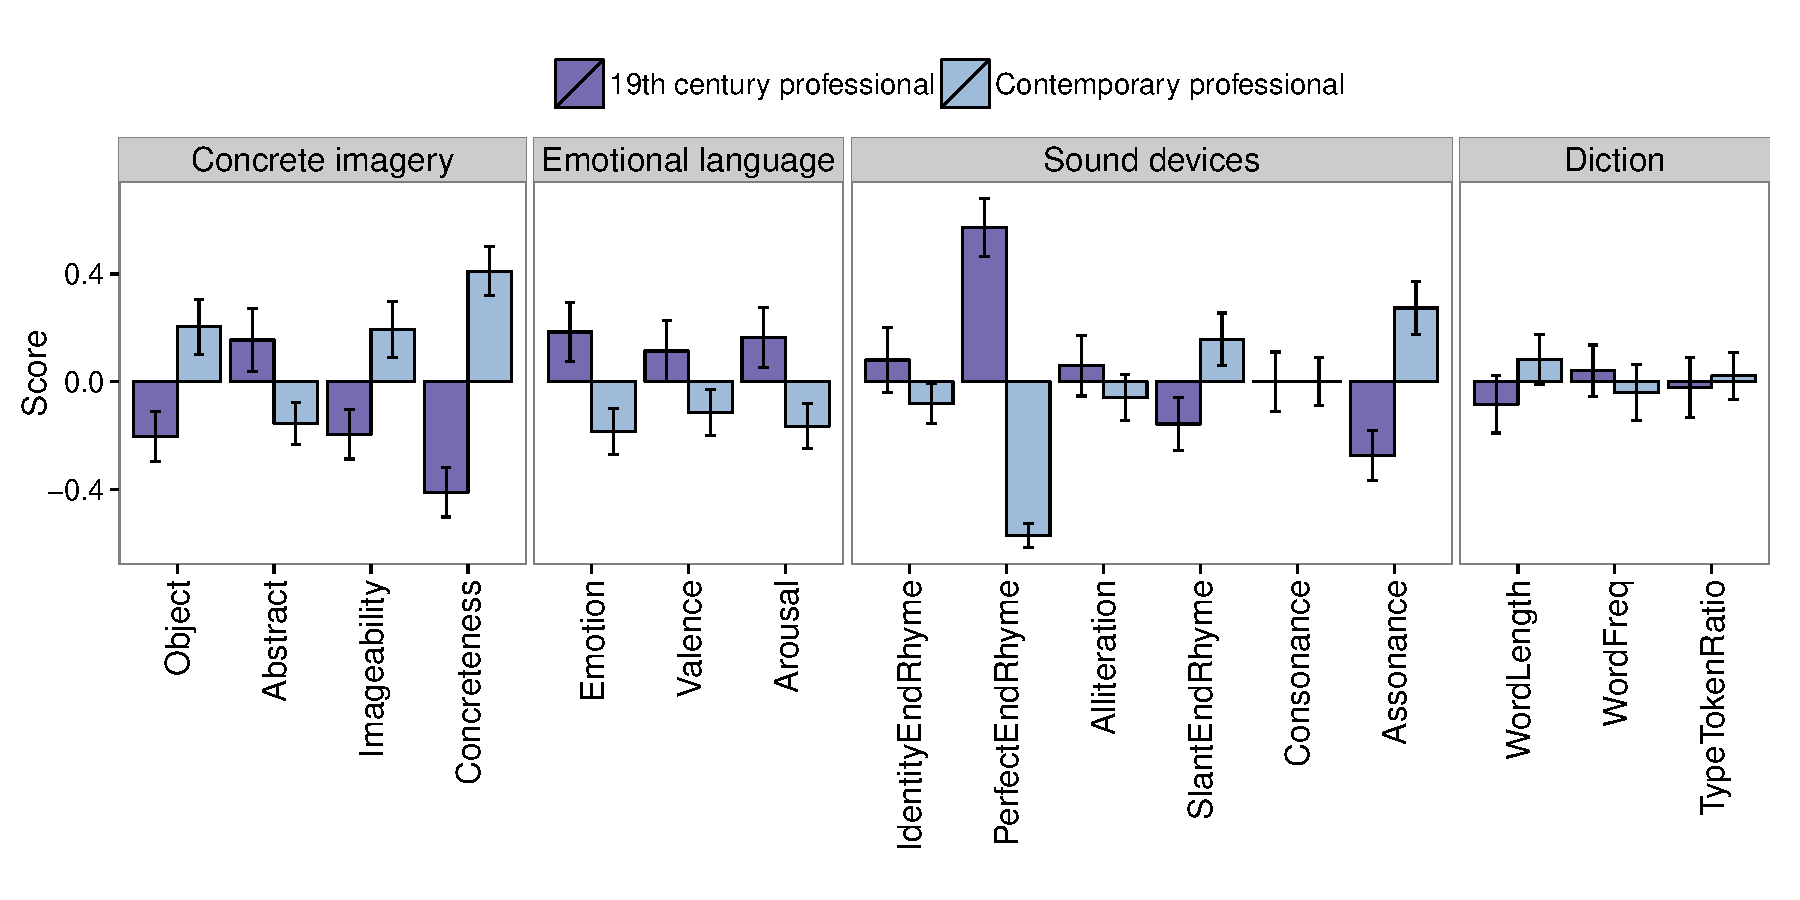
\includegraphics{../../Analyses/figure1.pdf}}
%\end{center}
\caption{Average z-scored feature scores for poems written by 19th century and contemporary professional poets. Error bars are standard error.} 
\label{fig1}
\end{figure}

We began with a simple analysis comparing the feature scores of poems written by 19th century professional poets (including Imagists) and contemporary professional poets (Figure~\ref{fig1}). With respect to the use of concrete imagery, we found that poems written by contemporary poets contained significantly more \emph{Object} words ($t(196.33) = 2.94, p < 0.005$) and significantly fewer \emph{Abstract} words ($t(172.68) = -2.21, p < 0.05$).
We also found that contemporary poems scored significantly higher on \emph{Concreteness} ($t(197.99) = 6.36, p < 0.00001$) as well as \emph{Imageability} ($t(195.18) = 2.80, p < 0.01$), suggesting that modern aesthetic standards are characterized by the presence of concrete imagery to a higher degree than 19th century poems.

In our analysis of emotional language, we found that poems written in the 19th century contain significantly more \emph{Emotion} words than contemporary poems ($t(187.24) = 2.65, p < 0.01$). This provides quantitative evidence that contemporary poets are less likely to make explicit references to emotions. 19th century and contemporary poems did not score significantly differently on \emph{Valence} ($t(185.14) = 1.62, p = 0.11$), suggesting that poets from both time periods used words with similar degrees of emotional positivity and negativity (although words in 19th century poems trended towards being slightly more positive). On the other hand, 19th century poems scored significantly higher on \emph{Arousal} ($t(183.60) = 2.36, p < 0.05$), suggesting that 19th century poets tend to use words that are more emotionally excited. Overall, these results suggest that contemporary poets are less likely to explicitly reference emotions and use more emotionally subdued language. 

The sound devices used by 19th century and contemporary poets also differ in interesting ways. 19th century poets used significantly more perfect end rhymes ($t(131.27) = 9.84, p < 0.00001$), which follows naturally from adherence to stricter poetic forms and rhyme schemes. On the other hand, contemporary poets developed ``new rhythms'' and new sound patterns by employing significantly more subtle devices such as slant end rhymes ($t(197.96) = 2.25, p < 0.05$) and assonance ($t(197.12) = 4.02, p <  0.00001$). The two groups of poems did not differ significantly in terms of their use of identity end rhymes, alliteration, or consonance.

Finally, our analysis of diction suggests that contrary to the tenet promoting the use of ``the language of common speech," contemporary professional poets did not use significantly shorter, more frequent, or more varied words than 19th century poets. This departure from our prediction highlights an interesting tension within the first tenet of the Imagist manifesto. While the language of common speech is desired, the pressure to employ ``the exact word" pushes contemporary poets to choose words with precise meanings, which tend to be words that are less frequently used because their meanings are only appropriate in highly specific contexts. 

Figure~\ref{fig1} shows the magnitude of the differences  between contemporary and 19th century poems for these $16$ features. The two sets of poems differ the most on \emph{PerfectEndRhyme} and \emph{Concreteness}, suggesting that the defining characteristic of professional poetry shifted from an emphasis on sound patterns to an emphasis on concrete imagery. These comparisons show that contemporary aesthetic standards are more consistent with Imagism sensibilities. However, it is unclear whether the Imagist movement was responsible for establishing this aesthetic, or whether the preference for more concrete imagery is the natural result of artistic tastes evolving over time. 

\cite{martindale1990clockwork} proposed that art naturally evolves to become more complex, because the pressure to be novel requires artists to create work with higher complexity. %Needs work
This complexity can manifest in higher concreteness, which may be partially responsible for the differences we observe in our analysis. If time is the best predictor for concreteness, then we would expect the degree of concreteness in a poem to be consistently higher the later it is written, regardless of the Imagism movement. If, on the other hand, Imagism is responsible for promoting concreteness as a critical characteristic of good poetry, then we would expect that poems written prior to the Imagism movement would be uniformly low on concreteness, while poems written after the movement would be uniformly high on concreteness. In other words, we would expect to see a shift in concreteness before and after the Imagism movement, without much systematic variation otherwise.

\begin{figure}
\scalebox{0.55}{\includegraphics{../../Analyses/figure2.pdf}}
\caption{Scatter plot of the birth years and concreteness of 200 poems. Each point represents a poem written by either a 19th century non-Imagist poet, 19th century Imagist poet, or a contemporary poet. Triangles represent poems written by poets involved in the Imagist movement. Red points represent poems written by poets who were either involved in the Imagist movement or may be influenced by the Imagist movement. From the visualization, we observe that there is an overall correlation between birth year and concreteness. However, we also observe that Imagist poets writing in the 19th century more closely resemble 20th century poets in terms of concreteness. Furthermore, within the red and blue points, there is no apparent positive correlation between birth year and concreteness.} 
\label{fig2}
\end{figure}

To test these two hypotheses, we obtained the birth years of each of the poets from Wikipedia and further classified the poets into more fine-grained time periods \footnote{Although the year in which each poem was written is a more accurate measure, this value is more difficult to obtain and can be adequately approximated by the poets' birth years for our purposes.}. Figure~\ref{fig2} shows the relationship between the poet's birth year and the poem's concreteness. 
%
We first tested whether the concreteness of a poem is correlated with the poet's birth year and found a significant correlation of $r = 0.386$ ($p < 0.0001$), suggesting that overall, more modern poets use more concrete words. We then tested whether this correlation is an artifact of the difference between 19th century and contemporary professional poets, or if it is consistent across time. We found that while contemporary poems had significantly higher concreteness scores than 19th century poems ($t(197.99 = -6.36), p < 0.00001$), there was no significant correlation between the poets' birth years and concreteness within these time periods ($r_{19th} = 0.05, p_{19th} =0.65$; $r_{contempt} = 0.16, p_{contemp} = 0.11$). To validate this result, we constructed a linear regression model with two predictors: the poet's birth year and a binary factor indicating whether the poem was written by a non-Imagist 19th century poet or an Imagist/contemporary poet. This model showed that the binary factor is a significant predictor of concreteness ($t = -2.85, p = 0.0048$), while birth year does not capture a significant amount of the residual variance ($t = 1.15, p= 0.25$). Our analysis suggests that the data more strongly supports the interpretation that Imagist poets writing in the 19th century used more concrete imagery than their peers, and that their style was in turn adopted by contemporary poets. In other words, concreteness is not simply a natural product of time, but rather the consequence of a highly concentrated and deliberate literary movement.

%Contemporary poets also use different types of sound devices from. These results suggest that contemporary poetry employs more concrete imagery and less abstract language. which is consistent with the idea that the poetic standards championed by Imagists continue to influence contemporary poets.

%\begin{figure}
%\scalebox{0.7}{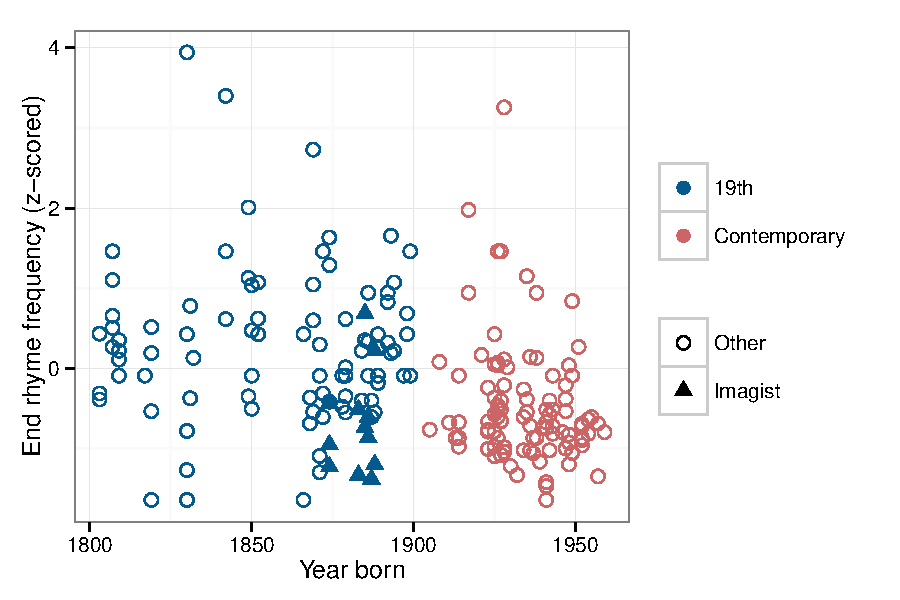
\includegraphics{../Analyses/figure4.pdf}}
%%\end{center}
%%\caption{Average marginal prior probability ratings for the three features given an animal category or a person category. Error bars are standard error over the $32$ items.} 
%\end{figure}

\section{Study 2: Contemporary professional vs amateur poets}
Our results from Study 1 suggest that the Imagism movement had a significant influence on the styles of contemporary professional poets. Is this influence also present in the works of contemporary amateur poets? Are literary movements only relevant to elite poets, or do they affect aesthetic standards across different levels of expertise? In this section, we explore the dynamics between professional and amateur poetry by examining the presence of Imagist ideals in poetry written by contemporary amateur poets. 

\subsection{Materials and methods}

$100$ poems were selected from amateur poets who submitted their work anonymously to a free and uncurated website, aptly called ``Amateur Writing'' (www.amateur-writing.com). At the time of selection, the website had over $2500$ amateur poem submissions by registered users. The website contains a diverse set of poems submitted by amateur writers with a wide range of experience and skill levels. We randomly selected poems from the website and corrected for misspellings and obvious grammatical errors in the poems to control for the effect of basic language skills. The final selection of amateur poems ranged from $21$ to $353$ words in length with an average length of $137.52$ words. 

%\begin{figure}
%\scalebox{0.45}{\includegraphics{../Analyses/figure2.pdf}}
%%\end{center}
%%\caption{Average marginal prior probability ratings for the three features given an animal category or a person category. Error bars are standard error over the $32$ items.} 
%\end{figure}

\subsection{Results}

\begin{figure}
\scalebox{0.38}{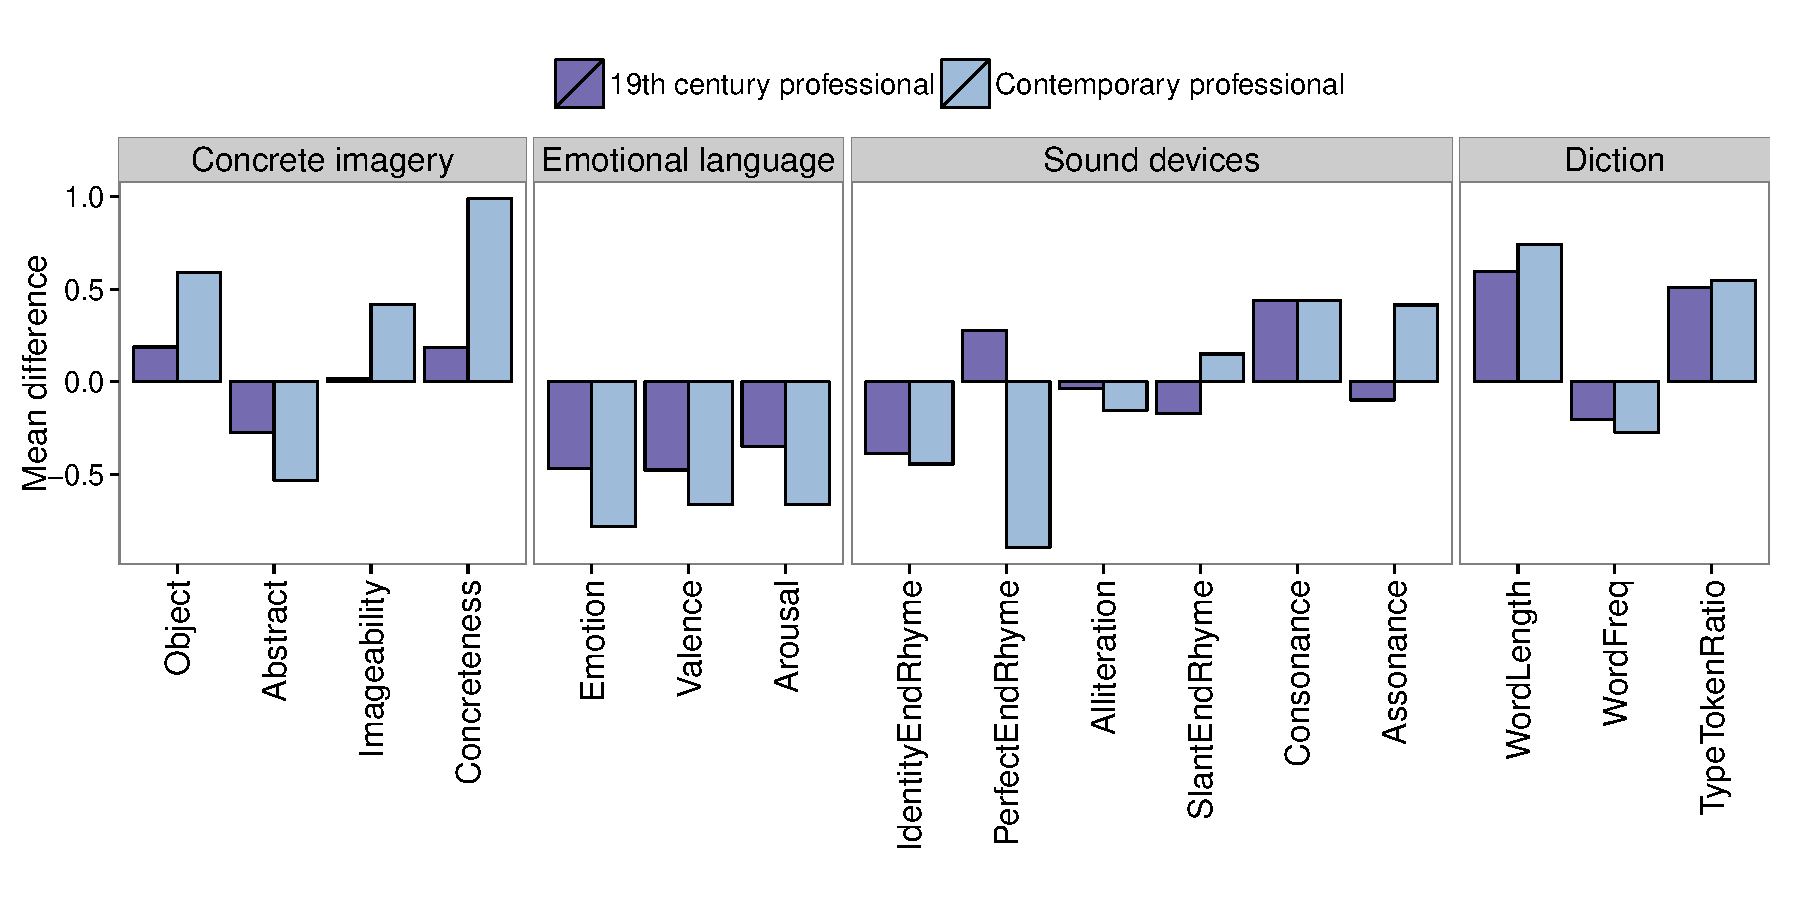
\includegraphics{../../Analyses/figure3-raw.pdf}}
%\end{center}
\caption{Difference in the feature score means between contemporary amateur poets and 19th century and contemporary professional poets. $0$ represents the mean feature scores for contemporary amateur poets. A positive dark blue bar indicates that 19th century professional poets scored higher on that feature than contemporary amateur poets. A negative pale blue bar indicates that contemporary professional poets scored lower on that feature than contemporary amateur poets. Overall, the dark blue bars tend to be shorter than the pale blue bars, indicating that contemporary amateur poems are more similar to 19th century professional poems than they are to contemporary professional poems.} 
\label{fig3}
\end{figure}

We implemented the 16 features described in Section 2 for the 100 amateur poems. To compare across the three sets of poems (19th century professional, contemporary professional, and contemporary amateur), each feature was standardized to have zero mean and unit variance across all 300 poems in our dataset. For each of the groups of poems, we computed the mean scores for each of the features. We then computed the difference between contemporary amateur poets' scores and the scores of 19th century and contemporary professional poets. Figure~\ref{fig3} shows the mean differences for each of the $16$ features. We see that professional poets from both eras tend to use more \emph{Object} words and fewer \emph{Abstract} words than amateur poets, as well as words with higher \emph{Imageability} and \emph{Concreteness}. Professional poets from both eras also tend to use fewer \emph{Emotion} words and words with lower \emph{Valence} and \emph{Arousal}. Amateur poets tend to use fewer \emph{PerfectEndRhymes} than 19th century professional poets, but still significantly more than contemporary professional poets. Professional poets from both eras also tend to use longer, less frequent words, and a more diverse vocabulary, than contemporary amateur poets.

Across all of these features, it appears that poems written by contemporary amateur poets exhibit significantly \emph{fewer} instances of Imagist ideals than poems written by either group of professional poets. Furthermore, poems written by amateur poets more closely resemble poems written by 19th century professional poets than their professional contemporaries. This can be seen from the fact that, regardless of directionality, the dark blue bars are shorter than the light blue bars ($t(27.36) = -3.35, p = 0.0023$), indicating that amateur poets are ``closer" in style to 19th century professional poets. Overall, these analyses suggest that the Imagist movement affected contemporary professional poets to a much greater degree than it did amateur poets---if it affected amateur poets at all.


%\section{Measures Comparison}
%Concreteness, imageability, and object words\\
%Valence, arousal, and emotion words\\
%``in literary usage, imagery  refers
% to images produced in the mind by language'' \citep{preminger1986princeton}.\\
%Auditory images:
%``Silently, easily we sway through braying traffic''


\section{Discussion}
In this paper, we quantified the aesthetic ideals of Imagism using computational linguistics techniques and evaluated the degree of conformity to these ideals in three sets of poems: poems written by 19th century professional poets, contemporary professional poets, and contemporary amateur poets. Our analyses reveal several interesting insights on Imagism and its effect on the modern literary aesthetic. First, poems written by contemporary professional poets exhibit significantly more features of Imagism than poems written by 19th century professional poets. This suggests that even though the Imagist movement itself was short-lived, the modern literary aesthetic has adopted Imagist ideals and moved away from the more abstract, emotional, and rhyme-schemed style of the 19th century. Second, while some theories of artistic change claim that the use of concrete imagery may be the natural consequence of time and the pressure to be novel \citep{martindale1990clockwork}, a more detailed analysis of concreteness suggests that the Imagist movement may have been responsible for promoting the use of concrete imagery, above and beyond a uniform pressure of time. 

Although contemporary professional poets have adopted Imagist ideals, we found that contemporary amateur poets use much fewer Imagist features. This result highlights the fact that literary styles can differ in critical ways across poets with different levels of expertise, even if they are writing in a similar time period. Several explanations may account for this difference. The first and perhaps most obvious explanation is that literary movements have a stronger influence on elite poets and do not tend to reach amateur poets. In fact, many literary movements in the late 19th century were targeted at professional writers and poets and intentionally created an atmosphere of exclusivity \citep{thacker2011imagist}.  A second explanation is that while amateur poets may seek to emulate elite poetry, it is more difficult for them to access the latest styles. As a result, their impression of good poetry is more likely to be shaped by the styles of the previous era. When amateur poets later produce poetry of their own, they tend to emulate these more ``outdated" styles. This explanation is closely related to \cite{simmel1957fashion}'s theory about fashion, where new fashion styles are constantly created by the elite (partly in order to distinguish themselves from the lower class), while the lower class emulates elite styles from the previous season and as a result lags a step behind. This theory predicts that amateur poets in the next century will write more like professional poets in this century, and that professional poets in the next century will develop a new style altogether. Although we currently lack the longitudinal data to test this theory, it offers interesting predictions that could be examined in future work.

While these two explanations both offer plausible reasons for why poems written by contemporary amateur poets exhibit fewer Imagist characteristics than contemporary professional poets, they fail to explain why contemporary amateur poets exhibit even fewer Imagist characteristics than 19th century professional poets. A third explanation addresses this issue, while making an interesting and rather controversial point about the nature of art and artistic change. ``Great poetry", the poet T.E. Hulme argued, ``always endeavors to arrest you, and to make you continuously see a physical thing, to prevent you from gliding through an abstract process." Perhaps the reason why amateur poets exhibit fewer features of Imagism than 19th century professional poets is because the Imagist aesthetic correlates with higher sophistication and is less likely to be mastered by amateur poets who lack the proper skill and training. Prior to the Imagist movement, professional and amateur poets wrote in a more similar style. As contemporary professional poets adopted the Imagist aesthetic, the gap between professional and amateur poets grew. It is possible that the style of contemporary professional poets is in some sense more ``advanced" than the style of 19th century professional poets, which in turn is more advanced than amateur poets. This explanation  suggests that the Imagist aesthetic not only happens to be the prominent aesthetic at the moment, but is a \emph{better} and more desirable aesthetic than the ones in the past. Indeed, modern writers are often given advice consistent with certain Imagist ideals. One of the most important and oft-repeated piece of advice for writers is the following: ``Show, don't tell.'' \cite{Burroway} interprets this as meaning: ``Use concrete, significant details that address the senses.''  \cite{Burroway} also writes, ``flat writing is\dots full of abstractions, generalizations, and judgments. When these are replaced with nouns that call up a sense image and with verbs that represent actions we can visualize, the writing comes alive.'' The rationale behind this type of advice is that effective imagery allows readers to bring in their own associations to understand and truly experience a new emotion. Many abstract concepts can be embodied or evoked by surprising imagery, and skilled poets and writers are able to pick out specific sensory details that evoke deeper abstractions and generalizations. In fact, the appeal of concrete imagery may have roots in processes that facilitate learning and memory. Research in psychology has shown that concrete noun pairs are easier to memorize than abstract noun pairs, which suggests that imagery can enhance the learning of word pairings \citep{pairing}. Other studies have shown that mental imagery facilitates relational association between concepts \citep{imagery}. Furthermore, \cite{neuro} found neural correlates that suggest that concrete nouns are processed differently in the brain than abstract nouns. One of the reasons why we find poetic imagery striking may be due to the psychological power of imagery to evoke rich associations formed by culture and personal experience. Not only are concrete images able to render the world in spectacular detail, they also provide windows into particular experiences on which readers can project their own perceptions and interpretations.

On the other hand, some views on artistic change would disagree with the claim that the contemporary imagery-based aesthetic is superior to poetic styles of the past. According to \cite{lowell1920tendencies}, ``Fundamental beliefs change art, but do not, necessarily, either improve or injure it. Great poetry has been written at every stage of the world's history, but Homer did not write like Dante, nor Dante like Shakespeare, nor Shakespeare like Edgar Allan Poe." This view suggests that while there are clear differences between ``great" and ``mediocre" poetry, the styles of great poetry vary significantly across different time periods, and there is not one single style that guarantees more ``greatness." If this is true, then are there objective features of greatness that are consistent across these diverse styles? It may be interesting to explore this possibility in future research by comparing ``great" and ``mediocre" poetry across time periods to extract common features that distinguish the two groups.

Regardless of any strong implications for the inherent value of Imagist ideals, our analysis supports the idea that Imagism has strongly influenced the ways in which modern professional poets think about literary writing. Our results suggest that professional poets are more likely to show, while amateur poets have a tendency to tell. This difference marks the most significant distinction between contemporary professional and amateur poetry in our analysis and may be an essential aspect of poetic beauty for the modern aesthetic.

In addition to our findings regarding concrete imagery, our analysis of sound devices also provides interesting insight into the current stylistic trends of contemporary professional poetry. Sound devices have a long history in poetry and are traditionally considered an important aspect of poetic craft. Research in psychology has also confirmed poets' intuitions about the powerful effects of sound patterns on perception and learning, showing that rhyme and   alliteration shape people's preferences and facilitate understanding \citep{aphorisms, reading}. However, contemporary professional poets now use these devices much less frequently than either 19th century poets or contemporary amateur poets. Sound devices that were traditionally important for mnemonic purposes are now more characteristic of amateur poetry. These results suggest that repetition of sound is becoming a less aesthetically significant poetic device among contemporary masters of poetry. Instead, imagistic patterns have largely displaced sound patterns and risen to power as the primary indicator of poetic language. 

The tools and methodology used in this work enabled us to operationalize the Imagist aesthetic and test its influence on a large number of poems. By critically examining the claim that Imagism gave rise to the modern aesthetic \citep{pratt1992imagism}, our work highlights the benefits of applying computational approaches to questions in the humanities. Without the fine-grained measurements that these tools provide, it would be difficult to tease apart the two competing hypotheses regarding the increasing levels of concreteness in poetry: whether it is a natural consequence of artistic evolution, or whether the Imagism movement was responsible for initiating and sustaining this change. Furthermore, we showed that the lexicons used in psycholinguistics and natural language processing  capture textual qualities that are important in literary analysis, such as imagery and sentiment, and that these measures yield sufficient signal to identify important trends in literary style. Finally, the computational nature of our analyses means that we can apply the same features and measurements to different set of poems and replicate or extend our findings. %For example, Study 1 and Study 2 used the same set of features to answer two different but related questions.
%: (1) how has Imagism influenced the contemporary literary aesthetic, and (2) how do amateur poets respond to literary change. 

Applying computational techniques to analyze literary style is not
a new idea: \citet{holmes1985analysis} discussed early on the benefits of
quantitative measures of style, and 
\citet{stamatatos2000automatic} used stylistic
measures to automatically classify texts into different genres and
authors.  More specifically in poetry,
\citet{Kaplan+Blei} developed a
computer program to visualize and compare the styles of different
American poets that we draw in this work; and
\citet{kao2012computational} and \citet{dalvean2013ranking} provide
earlier examination of the stylistic differences between professional and amateur poets.   

The results of our work are also consistent with recent computational
studies of literary style in prose. \citet{ashok}, for example, found 
lexical and syntactic features that correlate with literary
success in novels: more successful novels used more verbs  of cognition
and quotation and more discourse connectives, while less successful books used
clich\'{e}d words like ``love'' and more sentiment-laden words.

While we draw on the insights of such previous computational studies, 
our goal was somewhat more top-down, drawing measure directly
based on the tenets of a specific literary style,
and furthermore taking
%makes is that instead of
%generating many low-level and seemingly arbitrary features (such
%as the number of nouns, verbs, and commas in a poem) and using them
%to distinguish among various texts, we derived our measures directly
%based on the tenets of a specific literary style. Furthermore, we took
a historical perspective to investigate the impact that this
style has on later work. As a result, we hope that our findings are
interpretable and useful to scholars in the humanities, such that
the relationship between a tenet---``to present an image"---and its
operationalization---word-level \emph{concreteness} ratings---is
sufficiently clear.

%so that one more paragraph might talk about how this fits in with other
%digital humanities analysis, what the computational tools are that make this possible, etc.
%i guess the tools in this work are
%1) lexicons
%2) simple functions of words (frequencies, length, etc)
%3) computation of sound devices
%i�m not exactly sure what the paragraph says about them, or whether it�s worth 
%mentioning other DH papers or not, but a methodological conclusion is definitely worth adding.

While our analyses shed light on the contemporary literary aesthetic and its relationship to the Imagist movement, it leaves open many questions to investigate in future research. For example, of the many literary movements of the late 19th century, why did Imagism leave such a strong mark on modern poetic styles? Are contemporary amateur poets also beginning to adopt Imagist ideals, such that amateur poetry written more recently exhibit more concrete imagery and fewer sound devices than amateur poetry written in the last decade? Does modifying a professional poem to include fewer concrete words make modern readers perceive it to be less beautiful? Is it easier for people to memorize poems that contain more concrete words, in much the same way that it is easier to memorize poems with stricter rhyme schemes? These questions have important implications on theories of artistic change, the relationship between elite and mainstream literature, and the historical and psychological bases of aesthetic appreciation. Our work provides a novel way of using computational methods to begin answering these questions in an empirical and data-driven manner. By conducting a quantitative comparison of poetic style across time and expertise, we hope to contribute to a deeper understanding of the forces that shape and define great poetry throughout the ages.

%\begin{table}
%\centering
%
%\begin{tabular}{| l  r || l  r |} \hline
%\multicolumn{2}{| c ||}{\textbf{Professional }} & \multicolumn{2}{| c |}{\textbf{Amateur }}\\ \hline
%\textbf{Word} & \textbf{Count} & \textbf{Word} & \textbf{Count}\\\hline	
%tree	&29 &	thing&	40\\
%room	&20&	wall&	12\\
%thing	&18&	bed&	11\\
%grass	&17&	clock&	7\\
%wall	&14&	room&	7\\
%flower	&13&	tree&	6\\
%glass	 &13&	leave&	6\\
%floor	&13&	gift&5\\
%car	&12&	mirror&	4\\
%dirt	&11&	flower	&4 \\
%$[\dots]$ & 538 & $[\dots]$ & 103 \\\hline
%Proportion & $4.1\%$ & Proportion & $1.5\%$ \\
%Type count & 250 & Type count & 85\\ \hline
%\end{tabular}
%\caption{Concrete words}
%\end{table}
%
%\begin{table}
%\centering
%\begin{tabular}{| l  r || l  r |} \hline
%\multicolumn{2}{| c ||}{\textbf{Professional }} & \multicolumn{2}{| c |}{\textbf{Amateur }} \\ \hline
%\textbf{Word} & \textbf{Count} & \textbf{Word} & \textbf{Count}\\ \hline
%day	&40&	day&	54\\
%night	&31&	time&	33\\
%year	&25&	beauty&	25\\
%time	&20&	soul&	16\\
%death	&11&	night&	15\\
%new   &9	&new	&14\\
%morning &	8&	moment&	13\\
%childhood&	7&	christmas&	12\\
%hour	&7	&think&	11\\
%afternoon	&7	&future&	9 \\
%$[\dots]$ & 139 & $[\dots]$ & 143 \\\hline
%Proportion & $1.8\%$ & Proportion & $2.6\%$ \\
%Type count & 82 & Type count & 75 \\ \hline
%\end{tabular}
%\caption{Abstract words}
%\end{table}
%\begin{table}
%\centering
%\begin{tabular}{| l  r || l  r |} \hline
%\multicolumn{2}{| c ||}{\textbf{Professional }} & \multicolumn{2}{| c |}{\textbf{Amateur }}\\ \hline
%\textbf{Word} & \textbf{Count} & \textbf{Word} & \textbf{Count}\\\hline	
%all	&63&	all	&82\\
%nothing	&26&	never	&46\\
%never	&19&	always	&43\\
%always	&14&	nothing	&21\\
%every	&11&	every	&15\\
%any	&10&	forever	&14\\
%anything	&5&	anything	&7\\
%nobody	&5&	any	&6\\
%everything	&5&	everything	&5\\
%forever	&3&	everyone	&4 \\\hline
%Proportion & $ < 1\%$ & Proportion &$1.8\%$ \\ \hline
%\end{tabular}
%\caption{Generalization words}
%\end{table}

\section*{Acknowledgments}
We are deeply grateful for David Kaplan's generosity in sharing the code for the \emph{PoetryAnalyzer} program, on which a substantial part of our analysis is based. We also thank the reviewers of an earlier and shorter version of this paper presented at NAACL in 2012 for their helpful feedback.

\bibliographystyle{apa-good}
\bibliography{mybib}

\newpage
\section*{Appendix: List of poems}
\subsection*{19th century professional}

\begin{table}[h!]
\tiny
\begin{tabular}{lllll}
\toprule
No. & Poem title & Poet & Birth year & Imagist \\
\midrule
1 & From The Short Story What The Swallows Did & Louisa May Alcott & 1832 \\
2 & Turns And Movies: Zudora & Conrad Aiken & 1889 \\
3 & The Window & Conrad Aiken & 1889 \\
4 & Before an Examination & Stephen Vincent Benet & 1898 \\
5 & Lonely Burial & Stephen Vincent Benet & 1898 \\
6 & Knowledge & Louise Bogan & 1897 \\
7 & Weather & Ambrose Bierce & 1842 \\
8 & A Woman's Reason & Gelett Burgess & 1866 \\
9 & The Goops & Gelett Burgess & 1866 \\
10 & The Sheep & Ellis Parker Butler & 1869 \\
11 & Cupid Caught Napping & Ellis Parker Butler & 1869 \\
12 & In the desert & Stephen Crane & 1871 \\
13 & A god in wrath & Stephen Crane & 1871 \\
14 & Upon the road of my life & Stephen Crane & 1871 \\
15 & Once I knew a fine song & Stephen Crane & 1871 \\
16 & To Emily Dickinson & Hart Crane & 1899 \\
17 & Interior & Hart Crane & 1899 \\
18 & If I can stop one Heart from breaking & Emily Dickinson & 1830 \\
19 & I felt a Funeral in my Brain & Emily Dickinson & 1830 \\
20 & We lose -- because we win & Emily Dickinson & 1830 \\
21 & Going to Heaven! & Emily Dickinson & 1830 \\
22 & There is no Frigate like a Book & Emily Dickinson & 1830 \\
23 & Life's Tragedy & Paul Laurence Dunbar & 1872 \\
24 & Encouraged & Paul Laurence Dunbar & 1872 \\
25 & The Unlucky Apple & Paul Laurence Dunbar & 1872 \\
26 & Evadne & Hilda Doolittle & 1886 & yes \\
27 & Sheltered Garden & Hilda Doolittle & 1886 & yes \\
28 & A Noon Song & Henry Van Dyke & 1852 \\
29 & God of the Open Air & Henry Van Dyke & 1852 \\
30 & Indian Summer & Henry Van Dyke & 1852 \\
31 & Farewell and Thanksgiving & Mark van Doren & 1894 \\
32 & Macavity: The Mystery Cat & T. S. Eliot & 1888 & yes \\
33 & The Boston Evening Transcript & T. S. Eliot & 1888 & yes \\
34 & Give All To Love & Ralph Waldo Emerson & 1803 \\
35 & The Park & Ralph Waldo Emerson & 1803 \\
36 & Threnody & Ralph Waldo Emerson & 1803 \\
37 & The Road Not Taken & Robert Frost & 1874 \\
38 & Mending Wall & Robert Frost & 1874 \\
39 & My November Guest & Robert Frost & 1874 \\
40 & A Valentine & Eugene Field & 1850 \\
41 & Horace to phyllis & Eugene Field & 1850 \\
42 & The Boys & Oliver Wendell Holmes & 1809 \\
43 & The Organ-Blower & Oliver Wendell Holmes & 1809 \\
44 & End Of The World & Robinson Jeffers & 1887 \\
45 & Promise Of Peace & Robinson Jeffers & 1887 \\
46 & A Dream & Helen Hunt Jackson & 1831 \\
47 & My Tenants & Helen Hunt Jackson & 1831 \\
48 & Poets & Joyce Kilmer & 1886 \\
49 & The Rainy Day & Henry Wadsworth Longfellow & 1807 \\
50 & Woods in Winter & Henry Wadsworth Longfellow & 1807 \\
51 & The Three Kings & Henry Wadsworth Longfellow & 1807 \\
52 & Wapentake & Henry Wadsworth Longfellow & 1807 \\
53 & Before the Altar & Amy Lowell & 1874 & yes \\
54 & A Lady & Amy Lowell & 1874 & yes \\
55 & Anticipation & Amy Lowell & 1874 & yes \\
56 & Drying Their Wings & Vachel Lindsay & 1879 \\
57 & To Lady Jane & Vachel Lindsay & 1879 \\
58 & A Curse for Kings & Vachel Lindsay & 1879 \\
59 & City Visions & Emma Lazarus & 1849 \\
60 & The Taming of the Falcon & Emma Lazarus & 1849 \\
61 & A Dedication. To Charlotte Cushman & Sidney Lanier & 1842 \\
62 & To Beethoven & Sidney Lanier & 1842 \\
63 & A Red Flower & Claude McKay & 1889 \\
64 & On the Road & Claude McKay & 1889 \\
65 & Silence & Marianne Moore & 1887 & yes \\
66 & Love Is Not All & Edna St. Vincent Millay & 1892 \\
67 & The Suicide & Edna St. Vincent Millay & 1892 \\
68 & Griffy the Cooper & Edgar Lee Masters & 1868 \\
69 & Emily Sparks & Edgar Lee Masters & 1868 \\
70 & Poem in Prose & Archibald MacLeish & 1892 \\
71 & The Enthusiast & Herman Melville & 1819 \\
72 & Song & Edgar Allan Poe & 1809 \\
73 & The Valley Of Unrest & Edgar Allan Poe & 1809 \\
\bottomrule
\end{tabular}
\end{table}

\begin{table}[h!]
\tiny
\begin{tabular}{lllll}
\toprule
No. & Poem title & Poet & Birth year & Imagist \\
\midrule
74 & A Fairly Sad Tale & Dorothy Parker & 1893 \\
75 & Dilemma & Dorothy Parker & 1893 \\
76 & A Girl & Ezra Pound & 1885 & yes \\
77 & Song of the Bowmen of Shu & Ezra Pound & 1885 & yes \\
78 & Miniver Cheevy & Edwin Arlington Robinson & 1869 \\
79 & Lancelot & Edwin Arlington Robinson & 1869 \\
80 & Painted Head & John Crowe Ransom & 1888 \\
81 & Happiness & Carl Sandburg & 1878 \\
82 & Horse Fiddle & Carl Sandburg & 1878 \\
83 & The Idea Of Order At Key West & Wallace Stevens & 1879 \\
84 & Nomad Exquisite & Wallace Stevens & 1879 \\
85 & Do You Remember Once & Alan Seeger & 1886 \\
86 & To England at the Outbreak of the Balkan War & Alan Seeger & 1886 \\
87 & After Love & Sara Teasdale & 1884 \\
88 & The Years & Sara Teasdale & 1884 \\
89 & Prayer & Henry David Thoreau & 1817 \\
90 & Tell Me & Jean Toomer & 1894 \\
91 & O Captain! My Captain! & Walt Whitman & 1819 \\
92 & Beginners & Walt Whitman & 1819 \\
93 & Inscription & Walt Whitman & 1819 \\
94 & A Sort Of A Song & William Carlos Williams & 1883 & yes \\
95 & Portrait Of A Lady & William Carlos Williams & 1883 & yes \\
96 & A Golden Day & Ella Wheeler Wilcox & 1850 \\
97 & Our Blessings & Ella Wheeler Wilcox & 1850 \\
98 & A Word for the Hour & John Greenleaf Whittier & 1807 \\
99 & The Old Guitar & James Whitcomb Riley & 1849 \\
100 & Silver Filigree & Elinor Wylie & 1885 \\
\bottomrule
\end{tabular}
\end{table}

\subsection*{Contemporary professional}
\begin{table}[h!]
\tiny
\begin{tabular}{llll}

\toprule
No. & Poem title & Poet & Birth year \\
\midrule
1 & Riot Act April 29 1992 & Ai & 1947 \\
2 & Twenty-year Marriage & Ai & 1947 \\
3 & To Dorothy & Marvin Bell & 1937 \\
4 & To an Adolescent Weeping Willow & Marvin Bell & 1937 \\
5 & Dream Song 26: The glories of the world struck me & John Berryman & 1914 \\
6 & Dream Song 172: Your face broods & John Berryman & 1914 \\
7 & The Fish & Elizabeth Bishop & 1911 \\
8 & Warning to the Reader & Robert Bly & 1926 \\
9 & The Russian & Robert Bly & 1926 \\
10 & A Lovely Love & Gwendolyn Brooks & 1917 \\
11 & The Choir & Olga Broumas & 1949 \\
12 & at the cemetery walnut grove plantation south carolina 1989 & Lucille Clifton & 1936 \\
13 & scar & Lucille Clifton & 1936 \\
14 & Japan & Billy Collins & 1941 \\
15 & Writing in the Afterlife & Billy Collins & 1941 \\
16 & The Language & Robert Creeley & 1926 \\
17 & The Warning & Robert Creeley & 1926 \\
18 & Adultery & James Dickey & 1923 \\
19 & Tomatoes & Stephen Dobyns & 1941 \\
20 & Fragments & Stephen Dobyns & 1941 \\
21 & Wingfoot Lake & Rita Dove & 1952 \\
22 & The Stairway & Stephen Dunn & 1939 \\
23 & The Strange People & Louise Erdrich & 1954 \\
24 & New Vows & Louise Erdrich & 1954 \\
25 & Sexual Jealousy & Carol Frost & 1948 \\
26 & The Undressing & Carol Frost & 1948 \\
27 & To Kill a Deer & Carol Frost & 1948 \\
28 & Nostos & Louise Gluck & 1943 \\
29 & Celestial Music & Louise Gluck & 1943 \\
30 & How Simile Works & Albert Goldbarth & 1948 \\
31 & The Older Child & Kimiko Hahn & 1955 \\
32 & The Porcelain Couple & Donald Hall & 1928 \\
33 & Reuben Reuben & Michael S. Harper & 1938 \\
34 & Our Lady of the Snows & Robert Hass & 1941 \\
35 & The Image & Robert Hass & 1941 \\
36 & Those Winter Sundays & Robert Hayden & 1913 \\
37 & This Night & William Heyen & 1940 \\
38 & Playing Dead & Andrew Hudgins & 1951 \\
39 & Degrees Of Gray In Philipsburg & Richard Hugo & 1923 \\
40 & Absences & Donald Justice & 1925 \\
41 & Variations On A Text By Vallejo & Donald Justice & 1925 \\
42 & After Making Love we Hear Footsteps & Galway Kinnell & 1927 \\
\bottomrule
\end{tabular}
\end{table}

\begin{table}[h!]
\tiny
\begin{tabular}{llll}

\toprule
No. & Poem title & Poet & Birth year \\
\midrule
43 & Blackberry Eating & Galway Kinnell & 1927 \\
44 & Thrall & Carolyn Kizer & 1925 \\
45 & The Intruder & Carolyn Kizer & 1925 \\
46 & Facing It & Yusef Komunyakaa & 1947 \\
47 & Audacity of the Lower Gods & Yusef Komunyakaa & 1947 \\
48 & Heaven as Anus & Maxine Kumin & 1925 \\
49 & Nurture & Maxine Kumin & 1925 \\
50 & The Abduction & Stanley Kunitz & 1905 \\
51 & My Indigo & Li-Young Lee & 1957 \\
52 & Eating Alone & Li-Young Lee & 1957 \\
53 & The Mutes & Denise Levertov & 1923 \\
54 & Wedding-Ring & Denise Levertov & 1923 \\
55 & They Feed They Lion & Philip Levine & 1928 \\
56 & Animals Are Passing From Our Lives & Philip Levine & 1928 \\
57 & To Speak of Woe That Is in Marriage & Robert Lowell & 1917 \\
58 & Onions & William Matthews & 1942 \\
59 & Charles on Fire & James Merrill & 1926 \\
60 & b o d y & James Merrill & 1926 \\
61 & For the Anniversary of My Death & W.S. Merwin & 1927 \\
62 & When You Go Away & W.S. Merwin & 1927 \\
63 & Minor Miracle & Marilyn Nelson & 1946 \\
64 & The Small Vases from Hebron & Naomi Shihab Nye & 1952 \\
65 & Hello & Naomi Shihab Nye & 1952 \\
66 & Personal Poem & Frank O'Hara & 1926 \\
67 & Why I Am Not A Painter & Frank O'Hara & 1926 \\
68 & May-68 & Sharon Olds & 1942 \\
69 & University Hospital Boston & Mary Oliver & 1935 \\
70 & The Summer Day & Mary Oliver & 1935 \\
71 & Dearest Reader & Michael Palmer & 1943 \\
72 & Aubade: Some Peaches After Storm & Carl Phillips & 1959 \\
73 & Crossing The Water & Sylvia Plath & 1932 \\
74 & Power & Adrienne Rich & 1929 \\
75 & Root Cellar & Theodore Roethke & 1908 \\
76 & The Room of My Life & Anne Sexton & 1928 \\
77 & Her Kind & Anne Sexton & 1928 \\
78 & Fork & Charles Simic & 1938 \\
79 & My Noiseless Entourage & Charles Simic & 1938 \\
80 & Working Late & Louis Simpson & 1923 \\
81 & Cleaning a Fish & Dave Smith & 1942 \\
82 & Pacemaker & W.D. Snodgrass & 1926 \\
83 & Hay for the Horses & Gary Synder & 1930 \\
84 & Oranges & Gary Soto & 1952 \\
85 & Glass-Bottom Boat & Elizabeth Spires & 1952 \\
86 & Gin & David St. John & 1949 \\
87 & Traveling through the Dark & William Stafford & 1914 \\
88 & Notice What This Poem Is Not Doing & William Stafford & 1914 \\
89 & The Dancing & Gerald Stern & 1925 \\
90 & The Prediction & Mark Strand & 1934 \\
91 & The Night The Porch & Mark Strand & 1934 \\
92 & Letter & Jean Valentine & 1934 \\
93 & Year's End & Ellen Bryant Voigt & 1943 \\
94 & In Trackless Woods & Richard Wilbur & 1921 \\
95 & The Singing & C. K. Williams & 1936 \\
96 & More Blues and the Abstract Truth & C.D. Write & 1949 \\
97 & Approximately Forever & C.D. Wright & 1949 \\
98 & Clear Night & Charles Wright & 1935 \\
99 & Lying in a Hammock at William Duffy's Farm in Pine Island Minnesota & James Wright & 1927 \\
100 & A Blessing & James Wright & 1927 \\
\bottomrule
\end{tabular}
\end{table}

\subsection*{Contemporary amateur}
\begin{table}[h!]
\tiny
\begin{tabular}{llll}
\toprule
No. & Poem title & Poet & Birth year \\
\midrule
1 & Only but a dream & anonymous & n/a \\
2 & Dr. Heinz Doofenshmirtz & anonymous & n/a \\
3 & Freedom & anonymous & n/a \\
4 & The foolish man & anonymous & n/a \\
5 & Live for the moment & anonymous & n/a \\
6 & Eaten up & anonymous & n/a \\
7 & Gates of Goodbye & anonymous & n/a \\
8 & true beauty & anonymous & n/a \\
9 & A Walk in the Park & anonymous & n/a \\
10 & The two of them & anonymous & n/a \\
11 & Your life & anonymous & n/a \\
12 & Thing we have lost in fire & anonymous & n/a \\
13 & Mother Rabbit & anonymous & n/a \\
\bottomrule
\end{tabular}
\end{table}

\begin{table}
\tiny
\begin{tabular}{llll}
\toprule
No. & Poem title & Poet & Birth year \\
\midrule
14 & Aurora & anonymous & n/a \\
15 & Boy to a man & anonymous & n/a \\
16 & Goodbye poem & anonymous & n/a \\
17 & Read me & anonymous & n/a \\
18 & Angel eyes & anonymous & n/a \\
19 & Another Chapter & anonymous & n/a \\
20 & Self Reserved & anonymous & n/a \\
21 & Yet the sun still sleeps.  & anonymous & n/a \\
22 & Let love be as one & anonymous & n/a \\
23 & Charlotte Emily and Anne & anonymous & n/a \\
24 & Cappuccino & anonymous & n/a \\
25 & Pleasure trip & anonymous & n/a \\
26 & I thought I knew & anonymous & n/a \\
27 & Where is our fate formed? & anonymous & n/a \\
28 & Sometimes & anonymous & n/a \\
29 & Life & anonymous & n/a \\
30 & You can cry & anonymous & n/a \\
31 & Breaking heart & anonymous & n/a \\
32 & And a Merry Christmas to You & anonymous & n/a \\
33 & Everybody likes my clock & anonymous & n/a \\
34 & I nearly fell & anonymous & n/a \\
35 & Denial & anonymous & n/a \\
36 & Winter silence & anonymous & n/a \\
37 & Demons and scars & anonymous & n/a \\
38 & The first time I saw you.  & anonymous & n/a \\
39 & Sister & anonymous & n/a \\
40 & For Thee & anonymous & n/a \\
41 & Precious Lord & anonymous & n/a \\
42 & Love is like & anonymous & n/a \\
43 & Life2 & anonymous & n/a \\
44 & To Be Young And Naive & anonymous & n/a \\
45 & Why I love You & anonymous & n/a \\
46 & First Love & anonymous & n/a \\
47 & Miss You & anonymous & n/a \\
48 & THE END HAD COME & anonymous & n/a \\
49 & BABY OF POVERTY & anonymous & n/a \\
50 & Broken Home & anonymous & n/a \\
51 & My Thoughts On Love & anonymous & n/a \\
52 & Take Me Back & anonymous & n/a \\
53 & A Friend Is & anonymous & n/a \\
54 & THE GARDEN & anonymous & n/a \\
55 & Insomnia & anonymous & n/a \\
56 & Unrequited Love & anonymous & n/a \\
57 & Wavering & anonymous & n/a \\
58 & Garden of Shattered Dreams & anonymous & n/a \\
59 & Thinking Of You & anonymous & n/a \\
60 & My heart bleeds & anonymous & n/a \\
61 & Time Isn't Always a good thing & anonymous & n/a \\
62 & Is It Really Love & anonymous & n/a \\
63 & Same Ole' Story & anonymous & n/a \\
64 & Restored & anonymous & n/a \\
65 & Do You? & anonymous & n/a \\
66 & Adoption is Love & anonymous & n/a \\
67 & Road to Happiness & anonymous & n/a \\
68 & Untitled 1 & anonymous & n/a \\
69 & Reflection & anonymous & n/a \\
70 & A DREAM WITHIN A DREAM & anonymous & n/a \\
71 & Waiting & anonymous & n/a \\
72 & The War & anonymous & n/a \\
73 & On a Moonlit Night & anonymous & n/a \\
74 & Traipsing on Bantayan Shore & anonymous & n/a \\
75 & you are my angel & anonymous & n/a \\
76 & I Know & anonymous & n/a \\
77 & The Way That You Left Me & anonymous & n/a \\
78 & Waiting for Love & anonymous & n/a \\
79 & a love without good-byes & anonymous & n/a \\
80 & Wail of a wave & anonymous & n/a \\
81 & Your still here & anonymous & n/a \\
82 & Why? & anonymous & n/a \\
83 & Always on my mind. & anonymous & n/a \\
84 & Lonely in the dark room " & anonymous & n/a \\
85 & Untitled 2 & anonymous & n/a \\
86 & As One & anonymous & n/a \\
87 & life goes on & anonymous & n/a \\
88 & Everlasting Love & anonymous & n/a \\
89 & ethics of the blacks & anonymous & n/a \\
90 & Hazed Maze & anonymous & n/a \\
91 & ME AND YOU & anonymous & n/a \\
92 & When you left & anonymous & n/a \\
93 & MAGIC & anonymous & n/a \\
94 & TOGETHER. FOREVER! & anonymous & n/a \\
95 & YOU ARE MY EVERYTHING & anonymous & n/a \\
96 & Believe in Miracles ! & anonymous & n/a \\
97 & A Lie & anonymous & n/a \\
98 & I love you & anonymous & n/a \\
99 & It & anonymous & n/a \\
100 & Memories & anonymous & n/a \\
\bottomrule
\end{tabular}
\end{table}

\end{document}
